\documentclass[11pt]{article}

\usepackage[margin=1in]{geometry}
\usepackage[T1]{fontenc}
\usepackage{lmodern}
\usepackage{microtype}
\usepackage{amsmath}
\usepackage{graphicx}
\usepackage{subcaption}
\usepackage{float}
\usepackage{xcolor}
\usepackage[format=plain, font=small, labelfont={bf,color=accent}, skip=6pt]{caption}
\usepackage{titlesec}
\usepackage{fancyhdr}
\usepackage[colorlinks=true, linkcolor=accent, citecolor=accent, urlcolor=accent,
            pdftitle={Analysis of the Obstacle Potential Function},
            pdfauthor={}]{hyperref}

\definecolor{accent}{RGB}{20,60,110}

\titleformat{\section}
  {\normalfont\Large\bfseries\color{accent}}{\thesection}{0.6em}{}
\titleformat{\subsection}
  {\normalfont\large\bfseries\color{accent!85!black}}{\thesubsection}{0.6em}{}
\titlespacing*{\section}{0pt}{1.4em}{0.8em}
\titlespacing*{\subsection}{0pt}{1.0em}{0.5em}

\pagestyle{fancy}
\fancyhf{}
\renewcommand{\headrulewidth}{0.4pt}
\fancyhead[L]{\small\textcolor{accent}{Obstacle Potential Function}}
\fancyhead[R]{\small\thepage}

\title{\textcolor{accent}{\textbf{Analysis of the Obstacle Potential Function}}}
\author{}
\date{}

\begin{document}
\maketitle
\thispagestyle{fancy}

\begin{abstract}
\noindent
We study the obstacle potential $U_{obst}$ used for collision avoidance, examine the
resulting force field $\mathbf{F}=-\nabla U_{obst}$ around the obstacle vehicle, and
show that the relative-velocity term $\Delta v/\Delta v_{max}$ causes the force to grow
even as the vehicle recedes. We drop this term and re-examine the force response.
Finally, we consider an alternative pseudo-distance scaling -- combining the per-axis
time constants into a single, jointly velocity-scaled term -- and compare its behaviour
to the original formulation.
\end{abstract}

\section{Potential Function}

The obstacle potential is defined as

\begin{equation}
    U_{obst} = \frac{\lambda (\Delta v / \Delta v_{max})}
    {\left(1 - \dfrac{w}{\Delta x}\right)
    \sqrt{\left(\dfrac{\Delta x}{\tau(\Delta x, \Delta v_x)}\right)^2
    + \left(\dfrac{\Delta y}{\tau(\Delta y, \Delta v_y)}\right)^2}}
    \label{eq:potential}
\end{equation}

where the direction-dependent time constants are given by

\begin{align}
    \tau(\Delta x, \Delta v_x) &= \frac{(1 + \alpha \Delta v_x) + (\alpha \Delta v_x - 1)\tanh(-\Delta x \Delta v_x)}{2}\,\tau_x \\
    \tau(\Delta y, \Delta v_y) &= \frac{(1 + \alpha \Delta v_y) + (\alpha \Delta v_y - 1)\tanh(-\Delta y \Delta v_y)}{2}\,\tau_y
\end{align}

\noindent
Here $\Delta x, \Delta y$ are the relative position offsets to the obstacle vehicle, $\Delta v_x, \Delta v_y$ the relative velocities, $w$ the obstacle width, and $\lambda, \tau_x, \tau_y, \alpha, \Delta v_{max}$ are model parameters.

\subsection{Force Field}

The force field $\mathbf{F} = -\nabla U_{obst}$ resulting from Equation~\ref{eq:potential} is shown below under three relative-velocity scenarios: a pure lateral closing speed ($\Delta v_x$ only), a pure longitudinal closing speed ($\Delta v_y$ only), and both combined.

\begin{figure}[H]
    \centering
    \begin{subfigure}{0.32\textwidth}
        \centering
        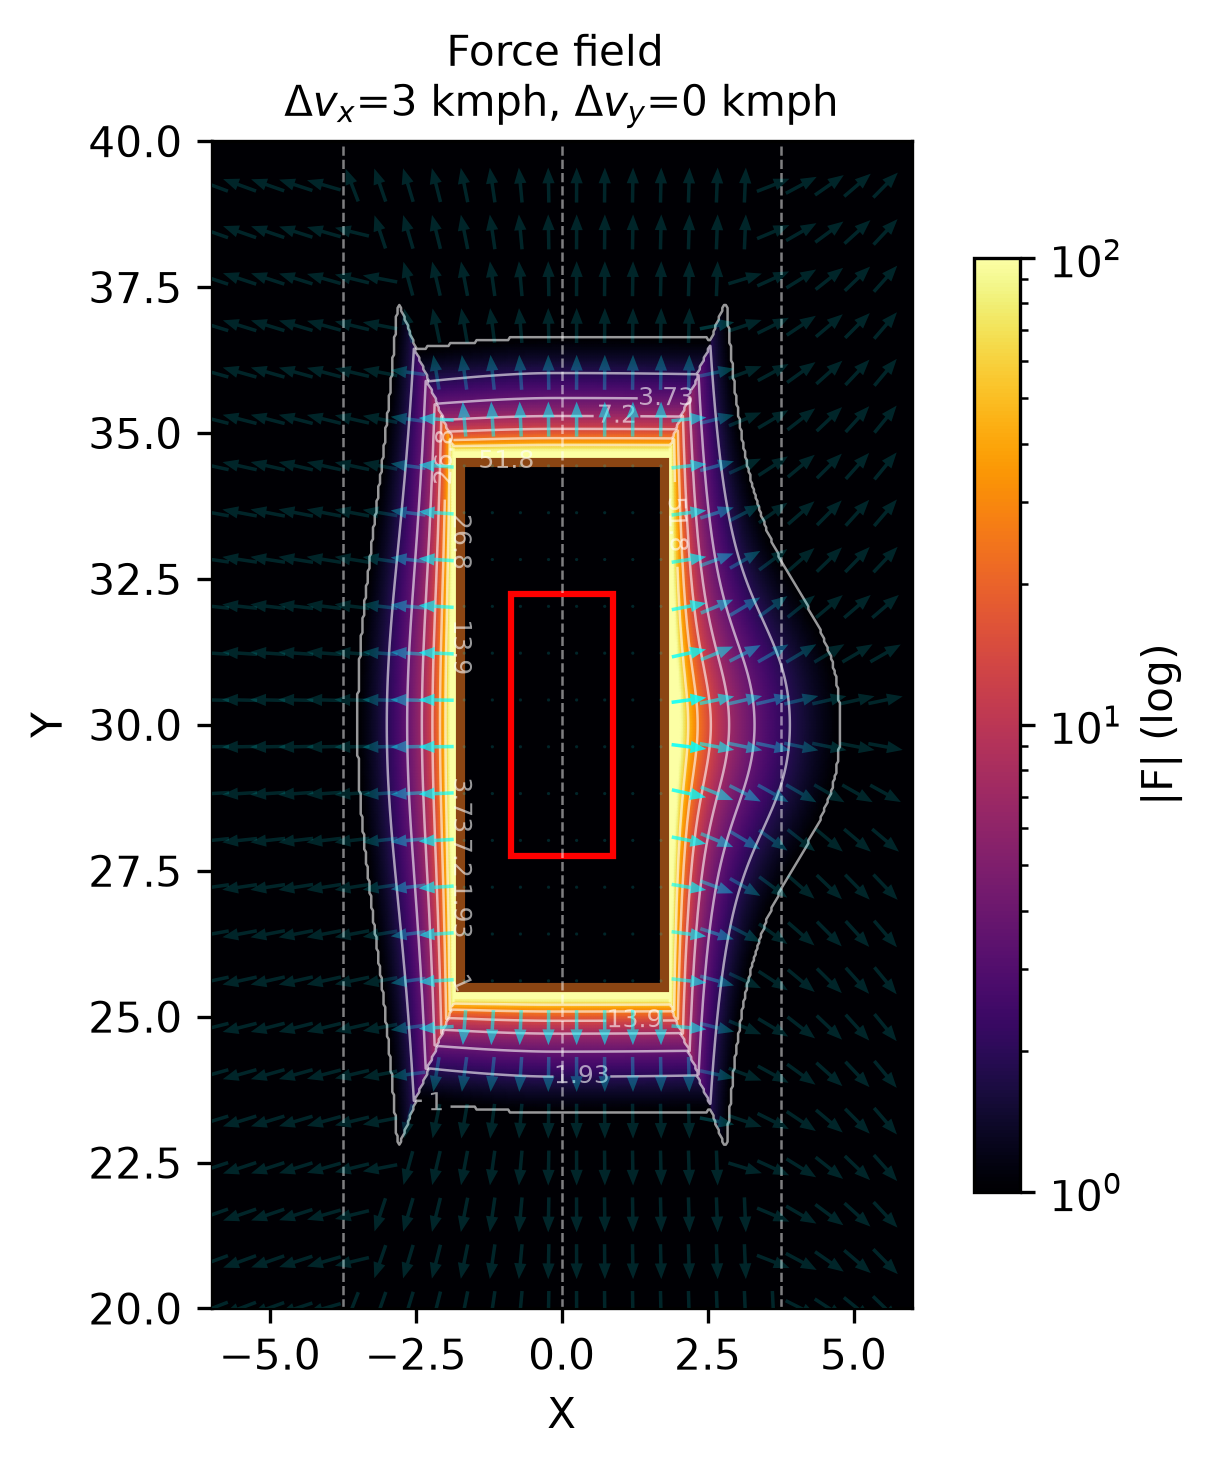
\includegraphics[height=4.2cm]{base_x.png}
        \caption{$\Delta v_x$ only}
    \end{subfigure}
    \begin{subfigure}{0.32\textwidth}
        \centering
        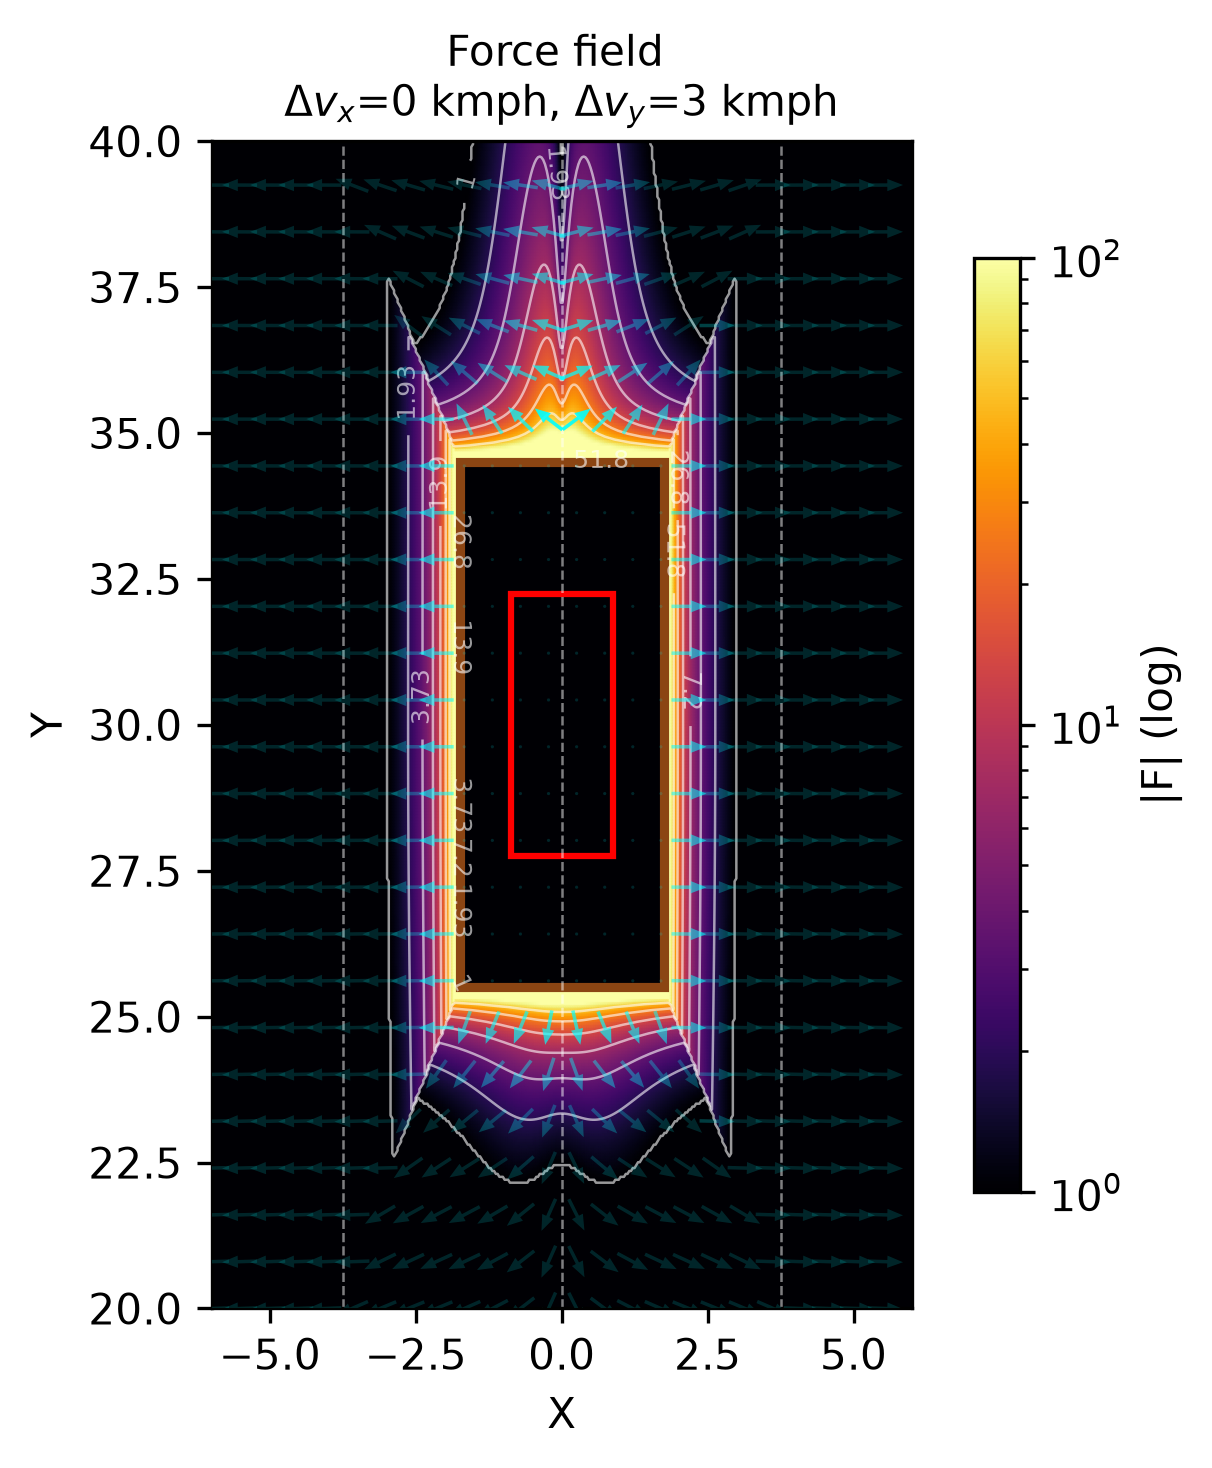
\includegraphics[height=4.2cm]{base_y.png}
        \caption{$\Delta v_y$ only}
    \end{subfigure}
    \begin{subfigure}{0.32\textwidth}
        \centering
        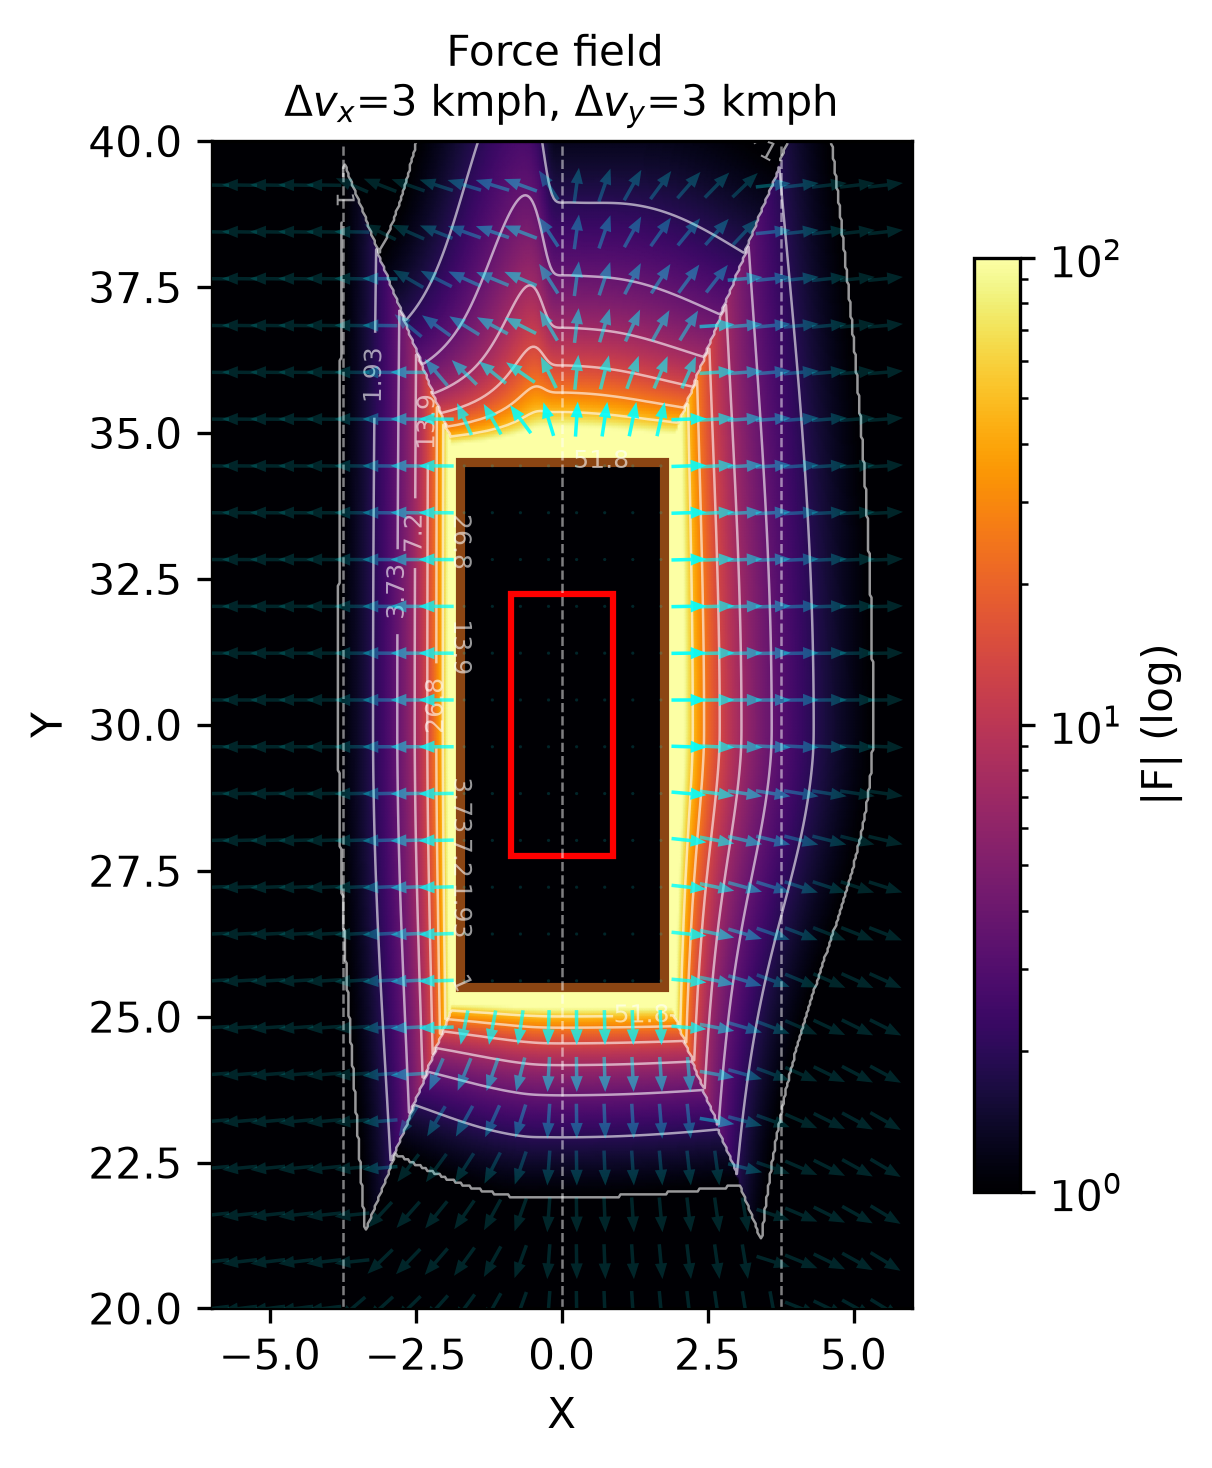
\includegraphics[height=4.2cm]{base_xy.png}
        \caption{Both combined}
    \end{subfigure}
    \caption{Force field of the potential in Equation~\ref{eq:potential}.}
    \label{fig:force_field}
\end{figure}

\section{Force at a Fixed Point vs. Relative Velocity}

To examine the velocity dependence of the force in more detail, we fix the position at $(x, y) = (3, 30)$ -- ahead of and to the side of the obstacle -- and sweep the relative velocity $v$ from $-10$ to $10$ kmph along several directions $(\Delta v_x, \Delta v_y)$, with $v$ scaling along each direction. Negative $v$ corresponds to the vehicle receding, positive $v$ to it closing.

\begin{figure}[H]
    \centering
    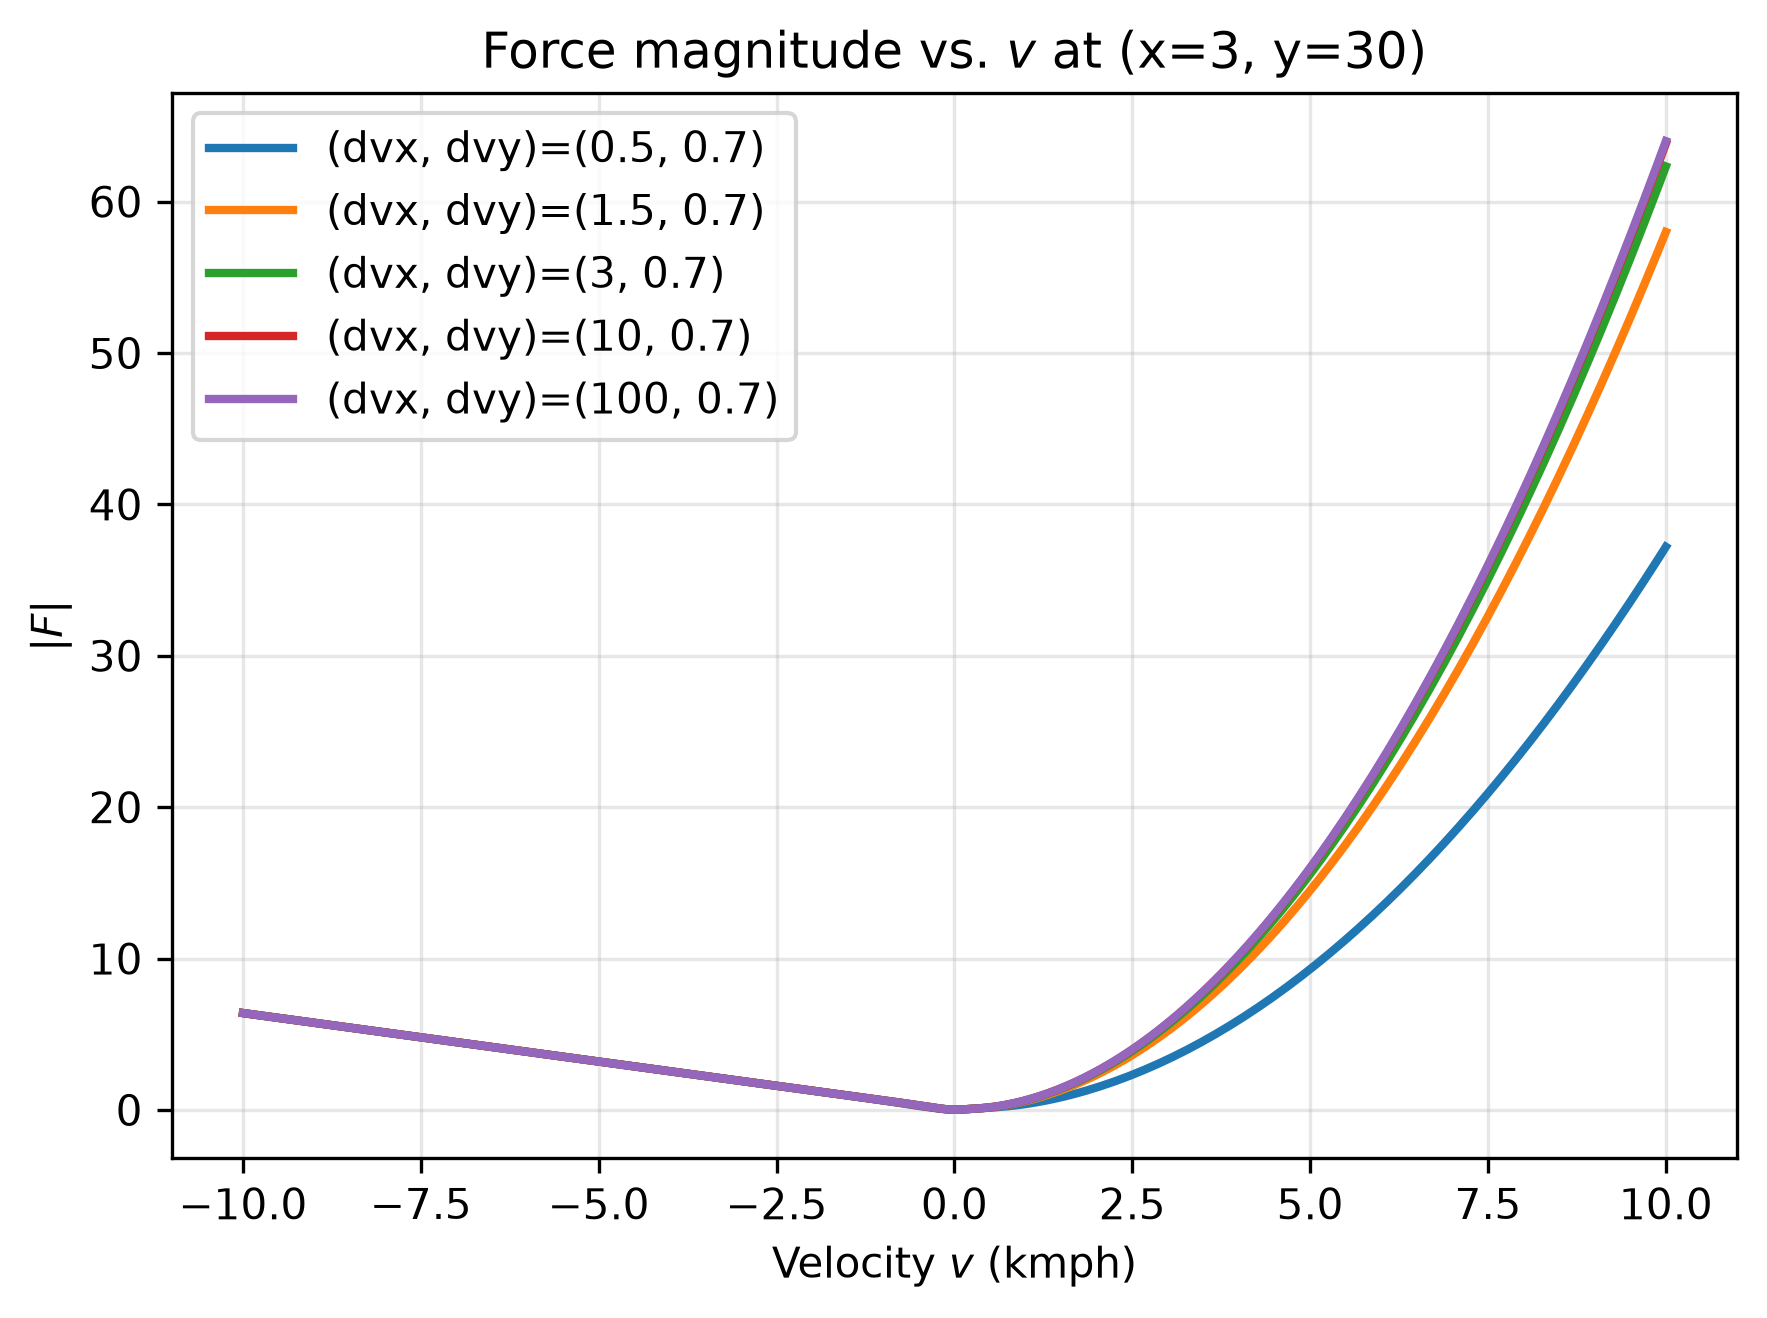
\includegraphics[width=0.7\linewidth]{base_vel.png}
    \caption{Force magnitude vs.\ relative velocity at $(x, y) = (3, 30)$.}
    \label{fig:base_vel}
\end{figure}

\section{Removing the \texorpdfstring{$\Delta v / \Delta v_{max}$}{Delta v / Delta v\_max} Term}

From Figure~\ref{fig:base_vel}, we observe that when the vehicle is receding ($v<0$), an increase in the magnitude of the relative velocity causes the force to increase as well. This is an undesirable effect, since a receding vehicle should not produce a growing repulsive force.

To avoid this behaviour, we drop the $\Delta v / \Delta v_{max}$ term from the original potential function in Equation~\ref{eq:potential}. Repeating the same experiment with this modified potential gives the plot below.

\begin{figure}[H]
    \centering
    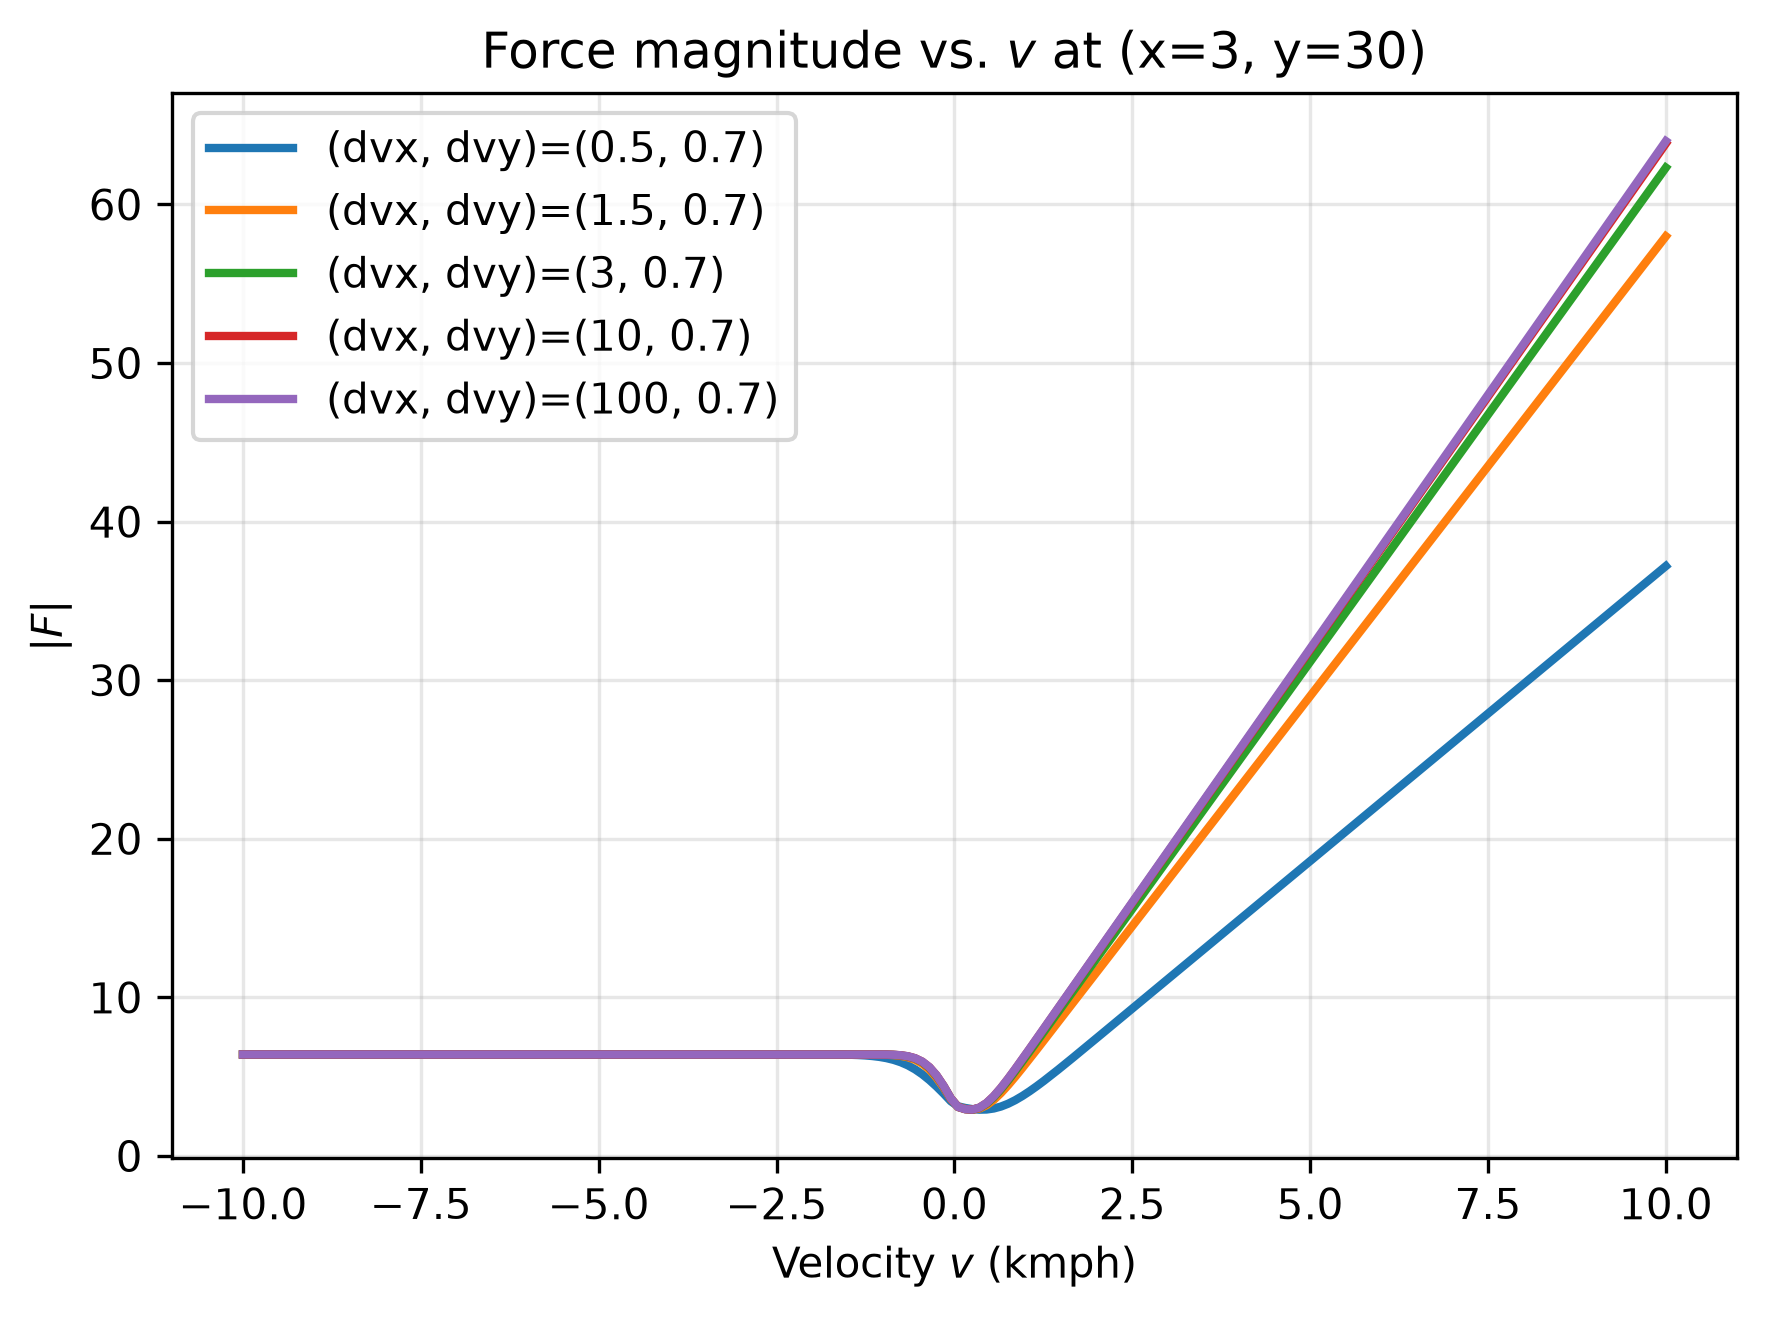
\includegraphics[width=0.7\linewidth]{base_vel_f.png}
    \caption{Force magnitude vs.\ relative velocity at $(x, y) = (3, 30)$, with the $\Delta v / \Delta v_{max}$ term removed.}
    \label{fig:base_vel_f}
\end{figure}

\section{An Alternative Pseudo-Distance Scaling}

The time constants $\tau(\Delta x, \Delta v_x)$ and $\tau(\Delta y, \Delta v_y)$ in Equation~\ref{eq:potential} modulate the $x$- and $y$-scales independently, each with its own relative velocity. As an alternative, we keep $\tau_x, \tau_y$ constant and instead scale the \emph{combined} pseudo-distance by a single factor that depends on the total relative speed and the closing rate:

\begin{equation}
    U_{obst}'' = \frac{\lambda \, g(\Delta x, \Delta y, \Delta v_x, \Delta v_y)}
    {\left(1 - \dfrac{w}{\Delta x}\right)
    \sqrt{\left(\dfrac{\Delta x}{\tau_x}\right)^2 + \left(\dfrac{\Delta y}{\tau_y}\right)^2}}
    \label{eq:potential_k9}
\end{equation}

\begin{align}
    g(\Delta x, \Delta y, \Delta v_x, \Delta v_y) &= \frac{(1 + \alpha |\Delta v|) + (\alpha |\Delta v| - 1)\tanh\!\big(-(\Delta v_x \Delta x + \Delta v_y \Delta y)\big)}{2}, \\
    |\Delta v| &= \sqrt{\Delta v_x^2 + \Delta v_y^2}
\end{align}

\noindent
As in Section~3, the $\Delta v/\Delta v_{max}$ prefactor is dropped. The resulting force field, under the same three velocity scenarios as Figure~\ref{fig:force_field}, is shown below.

\begin{figure}[H]
    \centering
    \begin{subfigure}{0.32\textwidth}
        \centering
        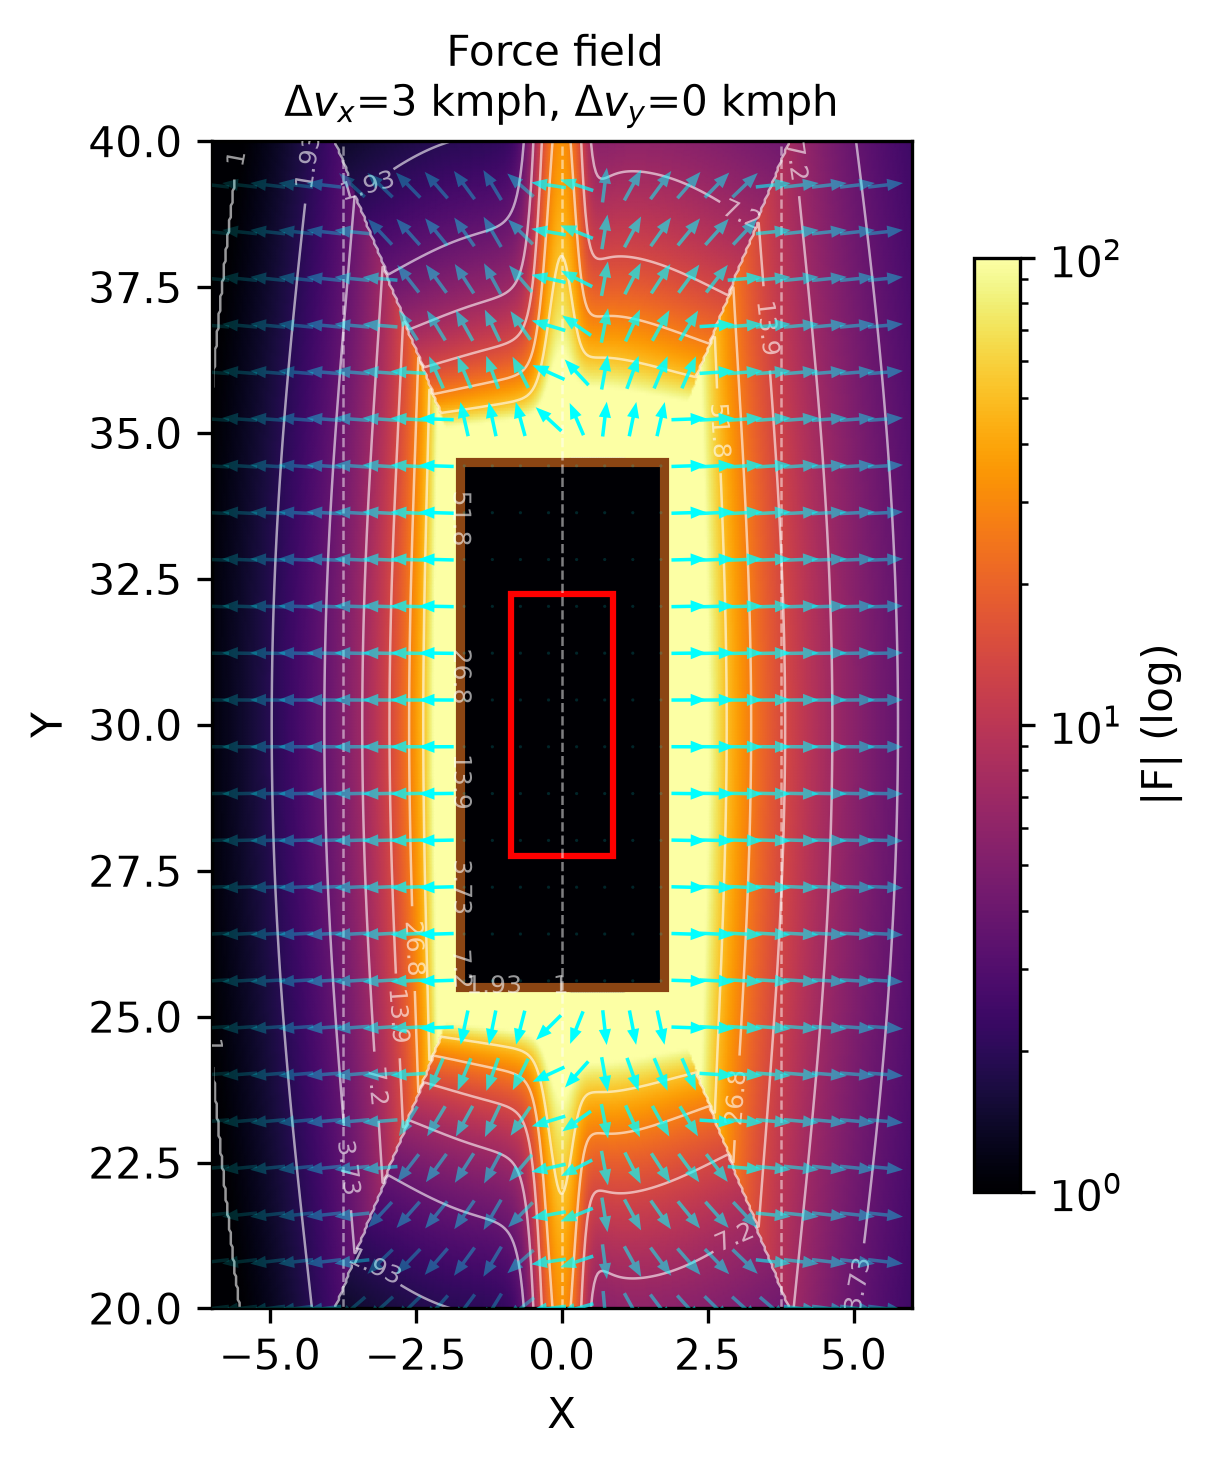
\includegraphics[height=4.2cm]{k9_base_x.png}
        \caption{$\Delta v_x$ only}
    \end{subfigure}
    \begin{subfigure}{0.32\textwidth}
        \centering
        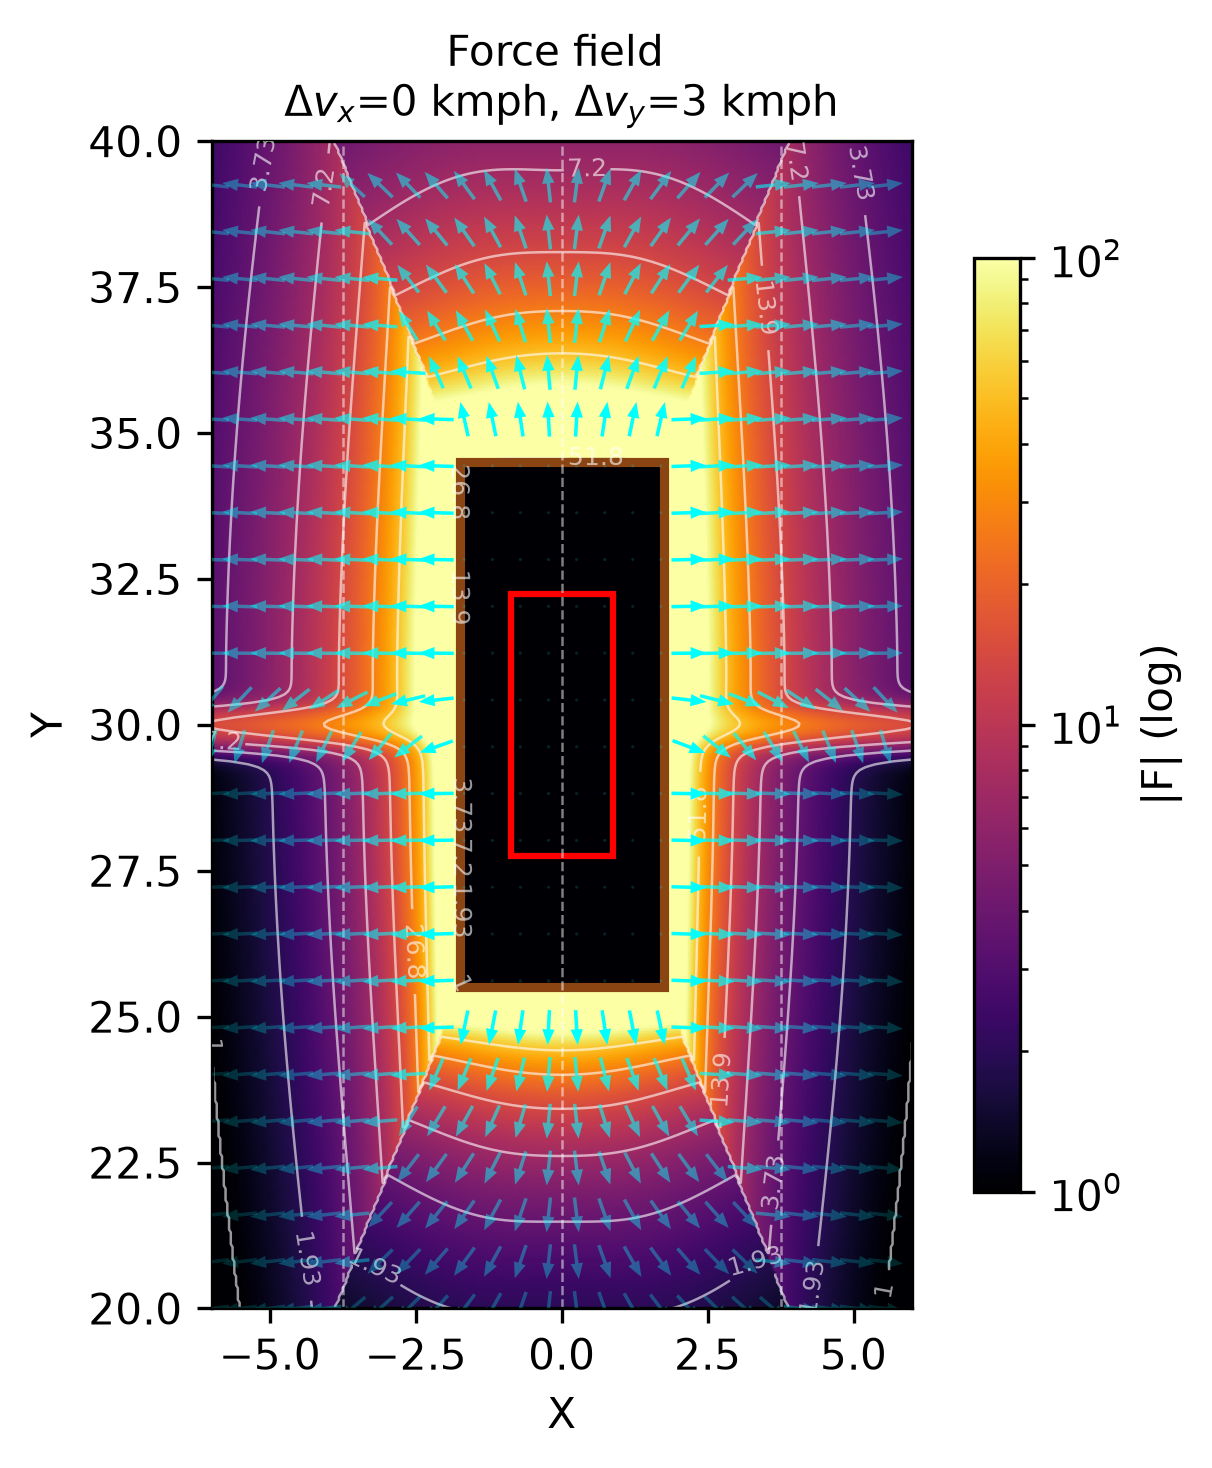
\includegraphics[height=4.2cm]{k9_base_y.png}
        \caption{$\Delta v_y$ only}
    \end{subfigure}
    \begin{subfigure}{0.32\textwidth}
        \centering
        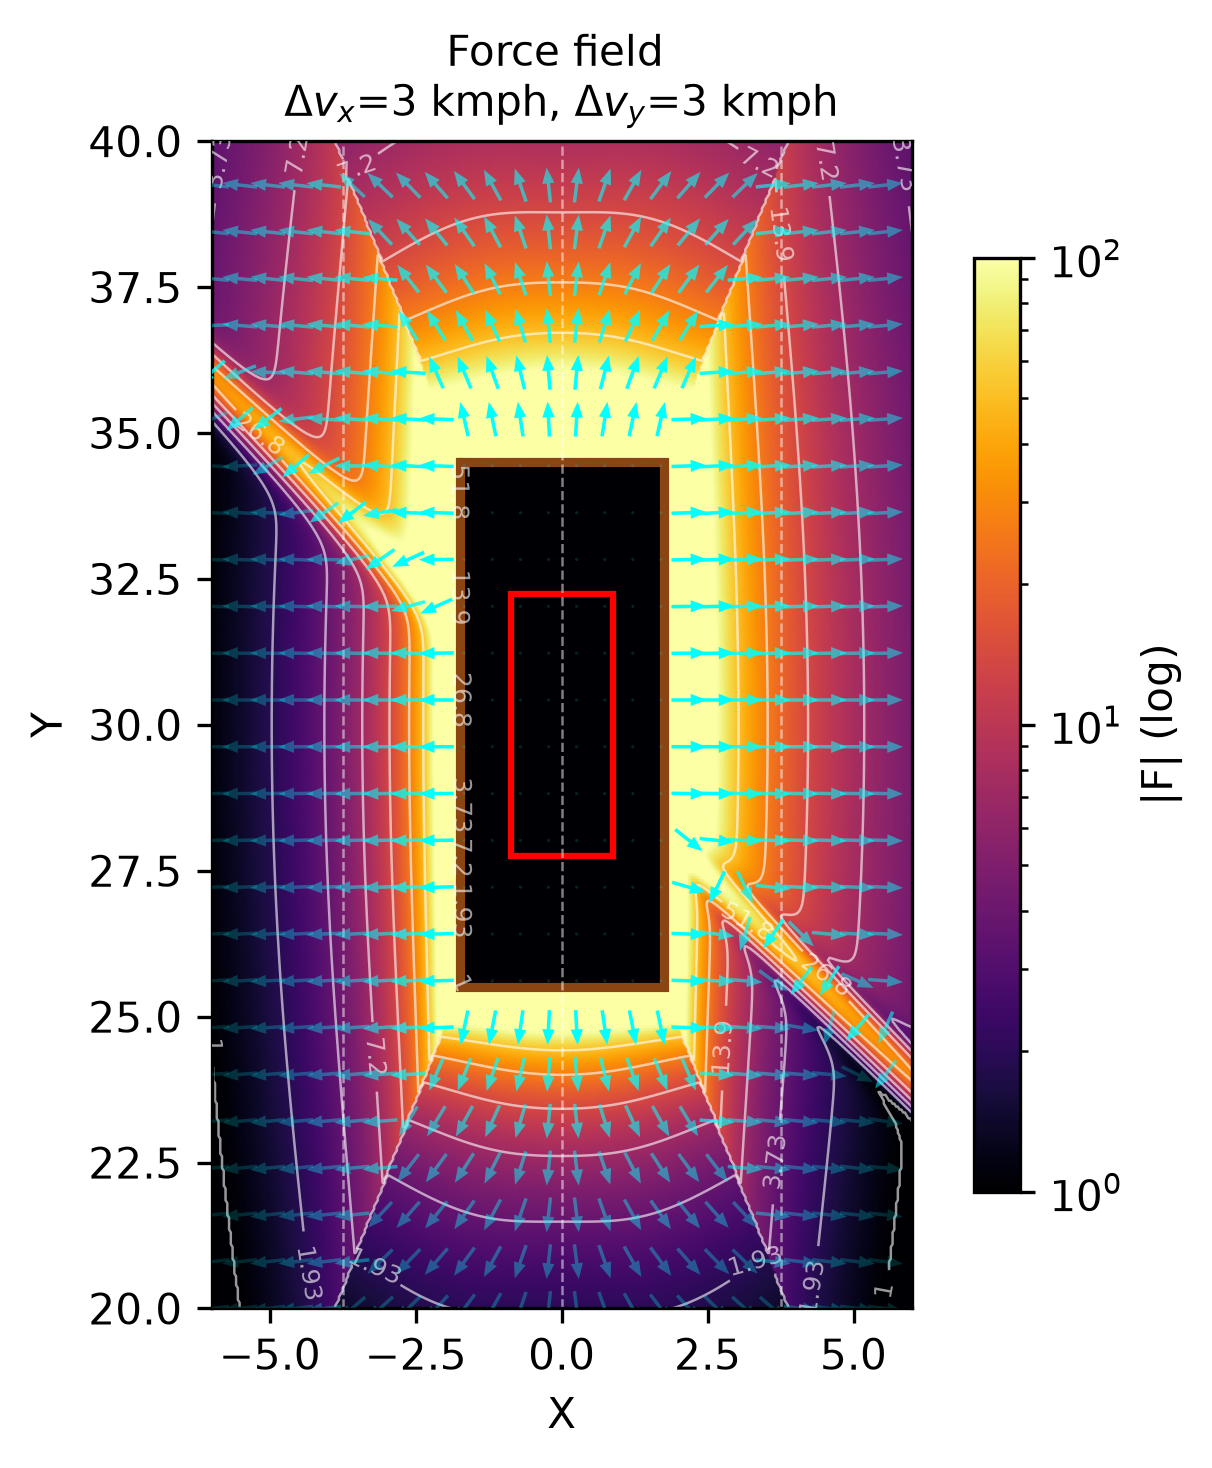
\includegraphics[height=4.2cm]{k9_base_xy.png}
        \caption{Both combined}
    \end{subfigure}
    \caption{Force field of the potential in Equation~\ref{eq:potential_k9}.}
    \label{fig:force_field_k9}
\end{figure}

Repeating the fixed-point sweep of Section~2 at $(x,y)=(3,30)$ with this potential gives:

\begin{figure}[H]
    \centering
    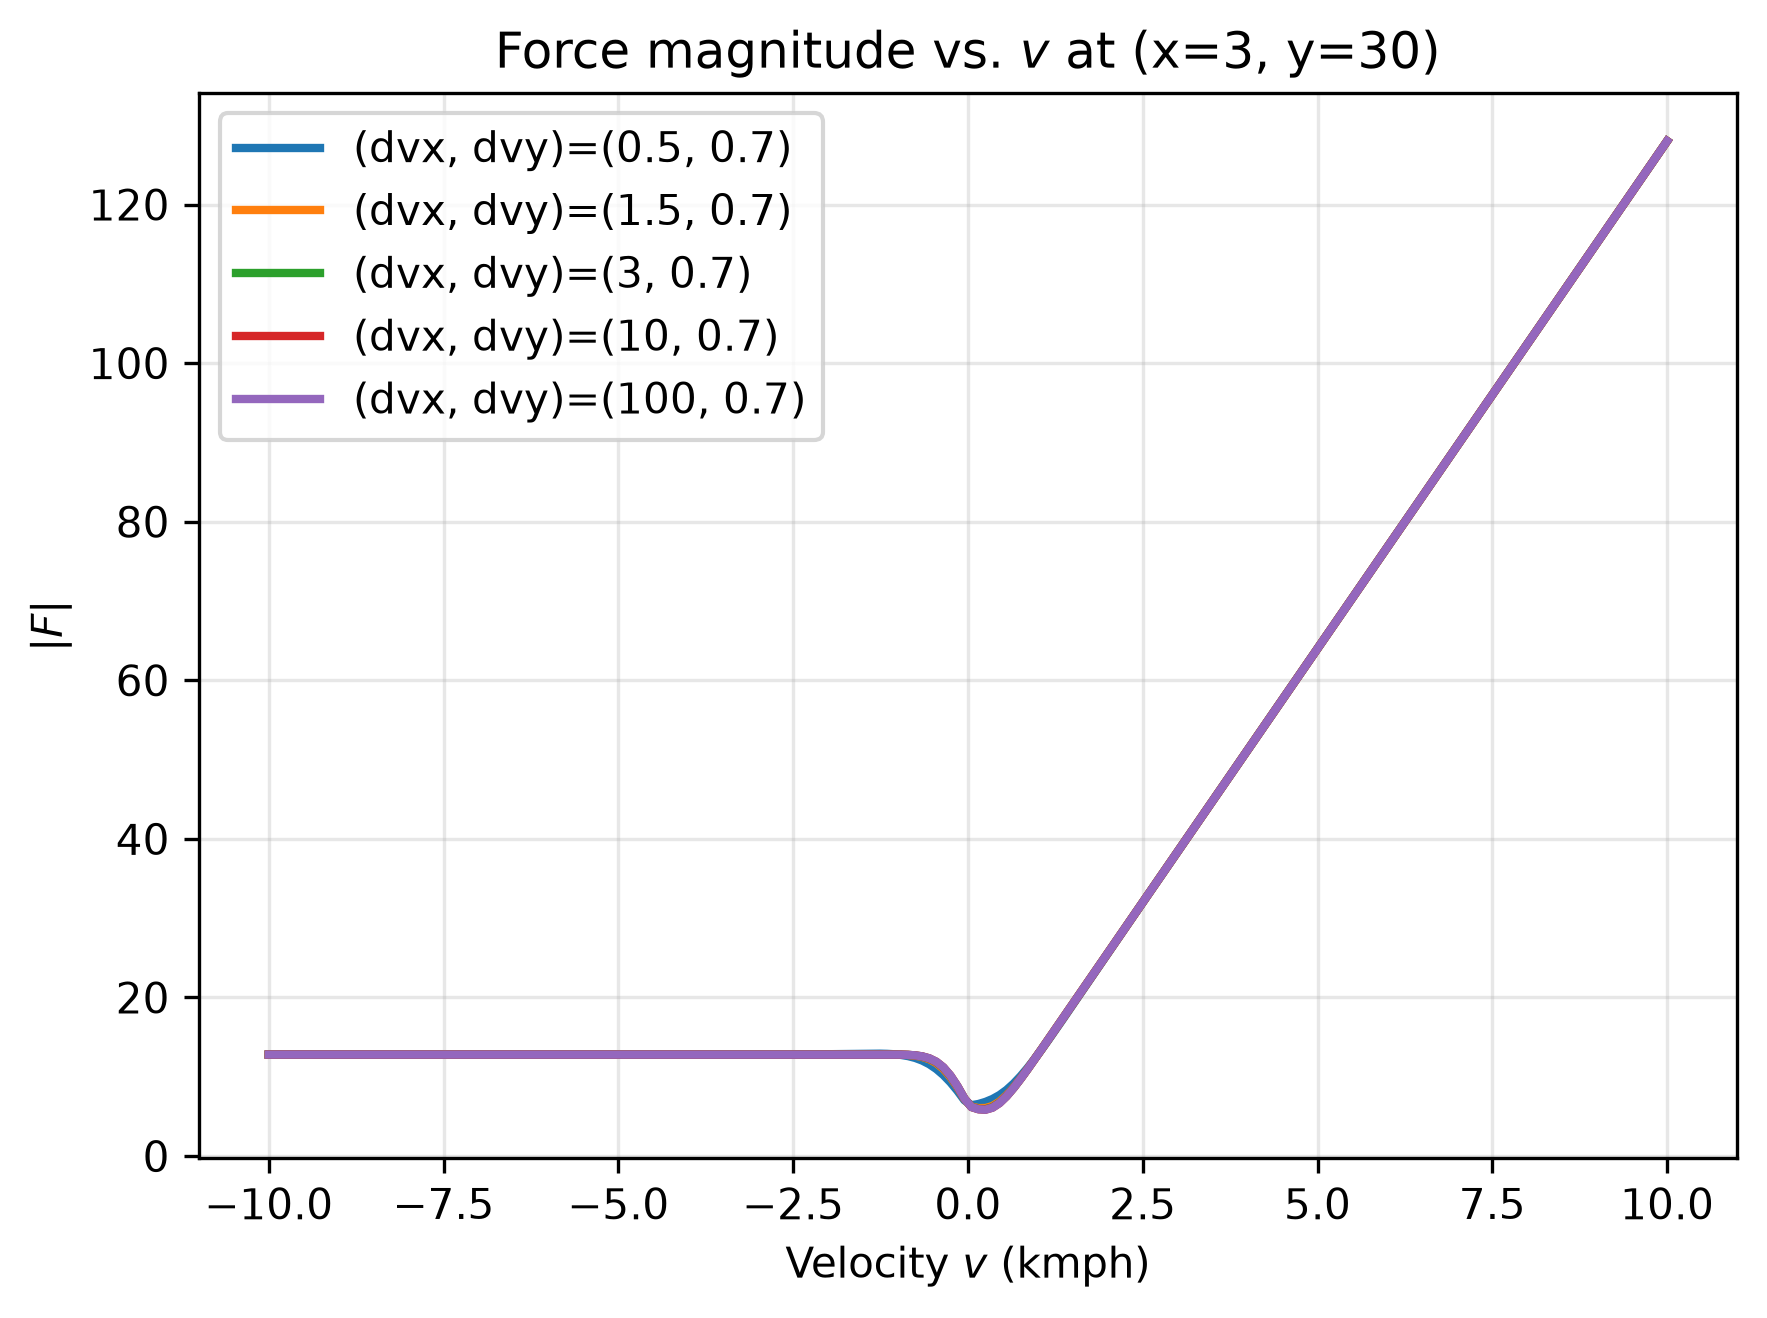
\includegraphics[width=0.7\linewidth]{k9_base_vel.png}
    \caption{Force magnitude vs.\ relative velocity at $(x, y) = (3, 30)$, under the potential in Equation~\ref{eq:potential_k9}.}
    \label{fig:k9_base_vel}
\end{figure}

Because the scaling factor $g$ depends only on the combined speed $|\Delta v|$ and the closing rate $\Delta v_x \Delta x + \Delta v_y \Delta y$, rather than on $\Delta v_x$ and $\Delta v_y$ separately, the five direction curves of Figure~\ref{fig:base_vel_f} collapse onto essentially one curve in Figure~\ref{fig:k9_base_vel}. We also note that the plateau at large negative $v$ persists here as well, which suggests that the receding-force effect discussed in Section~3 originates in the $\tanh$ modulation of the pseudo-distance itself, rather than in the $\Delta v/\Delta v_{max}$ prefactor alone.

\end{document}
